% !TEX root = ../main.tex
\graphicspath{ {./figures/} }

%%%%%%%%%%%%%%%%%%%%
\chapter{Evaluation}
%%%%%%%%%%%%%%%%%%%%

\TODO{Fix and improve all graphs, especially title and labels...}

The three algorithms will be evaluated based on their runtime and scalability. The evaluation will first cover synthetically generated graphs including randomly generated small and big graphs as well as corner cases, then graphs generated based on social behaviors, so-called social graphs, and finally graphs based on real-world datasets.

\section{Method}

\subsection{Generating Random Delegation Graphs}

For the first section, we built an algorithm, that builds a graph with n nodes, and then adds between zero and three delegations per node to random other nodes, ensuring that there are no delegation cycles without a sink. A better explanation of how these graphs are artificially constructed can be found in the Annex. \TODO{Create this annex} We acknowledge, that these assumptions may not be representative of real delegation graphs, where, as studies have shown, delegates tend to not delegate randomly, but to a subset of experts, such as TV personalities, thus centering power to one or few people. This approach also overlooks potential tendencies of voters, such as delegating to individuals they perceive as more competent or confident than them, or the tendency of power to concentrate among a few, very popular so-called "super-voters" \cite{klingVotingBehaviourPower2015}. These concerns are addressed in section XX, when we benchmark delegation graphs that are based on social graphs. 


\subsection{Preprocessing}

In order to be able to benchmark algorithms that resolve delegations, the input graphs need to be well-formed delegation graphs. In section XX and YY, we use graphs which are not well-formed delegation graphs out-of-the-box. This subsection details the process of how any arbitrary graphs, including undirected and unweighted graphs, can be turned into well-formed delegation graphs. An overview of this process is shown in \cref{fig:cleaning_process}.

\begin{figure}[t]
    \centering
    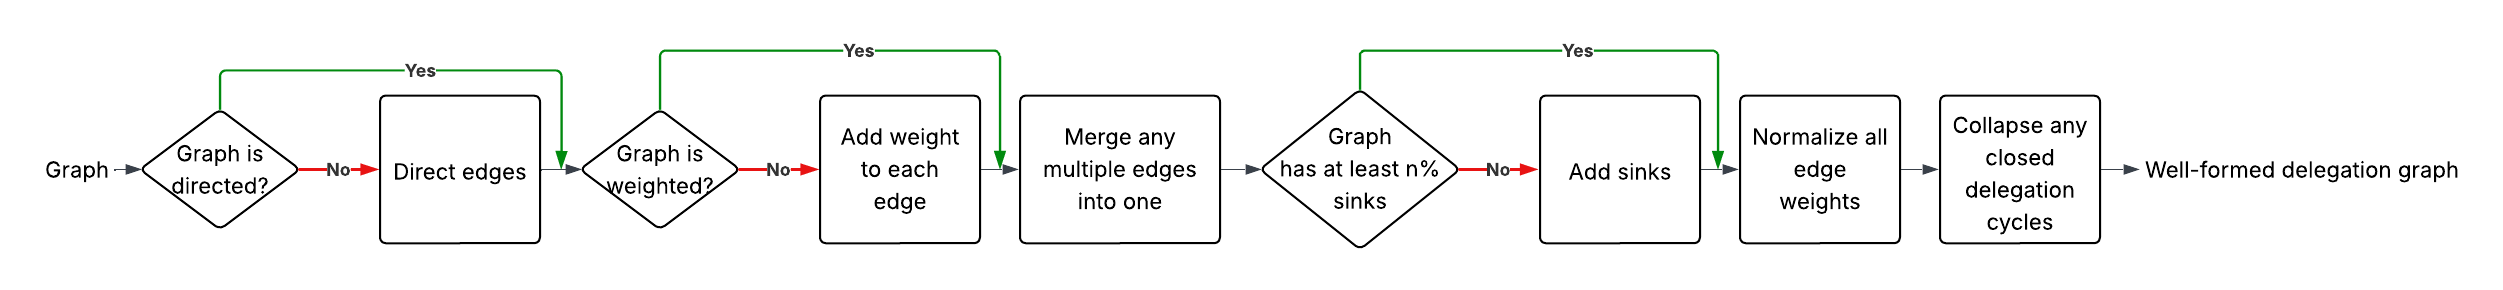
\includegraphics[width=\textwidth]{Thesis Evaluation Methodology Process.png}
    \caption{Process to clean any graph into a delegation graph.}
    \label{fig:cleaning_process}
\end{figure}

If the graph is undirected, is it given a direction. This is done arbitrarily, with the algorithm interpreting undirected edges in the shape $(u, v)$ as directed edges from u to v. If the algorithm fails to find a weight for an edge, it will also assign it a weight of one. Next, any multiple edges, so parallel edges going from the same node to the same node are merged, with any weights being added together. If less than $n\%$ of the graph's nodes are sinks, the algorithm randomly removes all outgoing delegations of delegators, turning them into sinks. By default this n value is 20, however depending on the use case it can be increased or decreased. After this, the algorithm searched for any closed delegation cycles, and collapses all it finds into a single sink node. Specifically, the algorithm searched for strongly connected components (STCCs) in the graph, so components of the graph where each node can reach each other node, and checks if it it is a closed delegation cycle, by checking if any of the nodes within this STCC to a node outside of the STCC. An exception to this are sinks who have no delegators, these are technically STCCs with no outgoing edges, however they are not closed delegation cycles. All closed delegation cycles are collapsed into a "lost" node, which means that any delegations to the cycle get re-directed to a specially created node. The resulting graph from this operation is a well-formed delegation graph, since all power that flows into closed delegation cycles now flows into a sink, so the graph is free of closed delegation cycles.

\subsection{Measurement}

Despite all algorithm's taking in put in inverse dict-of-dicts format, there may still be preprocessing necessary. While the iterative solver can use the inverse dict-of-dicts directly, using it as a lookup table as it spreads power around the graph, the other solver require the system of linear equations in specific formats, which need to be set up from the inverse dict-of-dicts input. Including such set-up time in benchmarks may be misleading, as this time is not spent on actually resolving delegations, thus we separated the set-up and resolving, and in the benchmarks only the time spent actually resolving the delegations is used; any set-up time is ignored. Nevertheless, in practice, the set-up time can be a relevant factor—depending on the use case and data format—when choosing between different approaches or implementations. The set-up procedures required for each implementation are described in more detail in the sections below.

To minimize the impact of background noise and measurement fluctuations on the benchmarks, algorithms with very short runtimes were executed multiple times, and the average runtime was recorded. The recorded runtimes always indicate just the runtime for the algorithms to resolve the delegations, times for set-up, such as the time for building the linear program, were not included. 

% cont here, merge the old benchmark stuff into these new sections, and add the new data

\section{Synthetic Graphs}

\subsection{Small Graphs}
\label{subsec:small_graphs}

\begin{figure}[t]
    \centering
    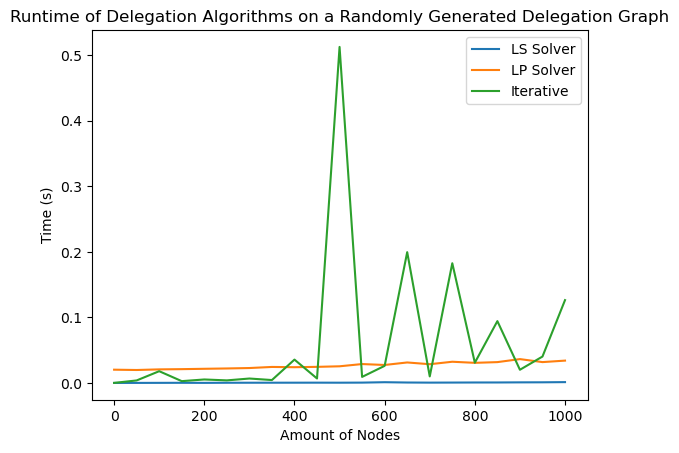
\includegraphics[width=0.4\textwidth]{0-1000_random}
    \caption{Runtime of delegation algorithms on a randomly generated delegation graph.}
    \label{fig:random-small}
\end{figure}

In order to explore the three algorithm's behavior on small graphs, we used the graph generator to generate graphs with zero to 1000 nodes. \Cref{fig:random-small} shows the results of this benchmark.

We can see, that the LS Implementation, optimized for sparse matrices, outperforms the other two algorithms. Its growth in runtime is so small, that the line looks to be staying flat on the x-axis. However, with a graph of 1000 nodes, its runtime is about 0.01 seconds. Both the LS and LP implementation display a rather steady, yet growing runtime. The LP solver seems to have some overhead, since even when the graph has zero nodes, it has a runtime of about 0.02 seconds.

Furthermore, we can interestingly observe large spikes in the runtime of the iterative approach. Exploring this more closely, we find that the graph with 11 nodes takes the iterative algorithm a lot more time than the graph with 10 or 12 nodes, as shown in \cref{fig:random-tiny}. At 10 nodes, the runtime of the iterative algorithm is just about 0.004 seconds, at 12 nodes it is 0.001 seconds, so even slightly faster than the slightly smaller graph, but when the graph has 11 nodes, the runtime skyrockets to about 0.056 seconds.

\begin{figure}[t]
    \centering
    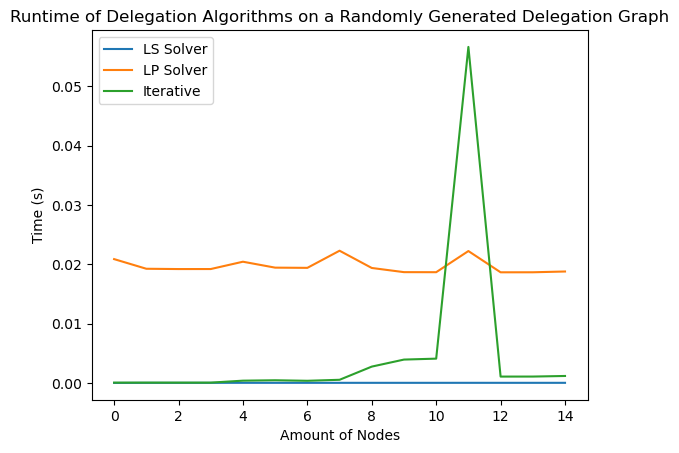
\includegraphics[width=0.4\textwidth]{0-15_random}
    \caption{Runtime of delegation algorithms on a randomly generated delegation graph.}
    \label{fig:random-tiny}
\end{figure}

A possible explanation for this spike may be, that when the graph has 10 and 12 nodes, it iterates only 758 and 170 times respectively, before cutting off, while when it has 11 nodes it iterates 8735 times before cutting off. \Cref{fig:random-11and12} shows the two graphs with 11 and 12 nodes.

\begin{figure}[t]
    \centering
    \begin{subfigure}[t]{0.45\textwidth}
        \centering
        \fbox{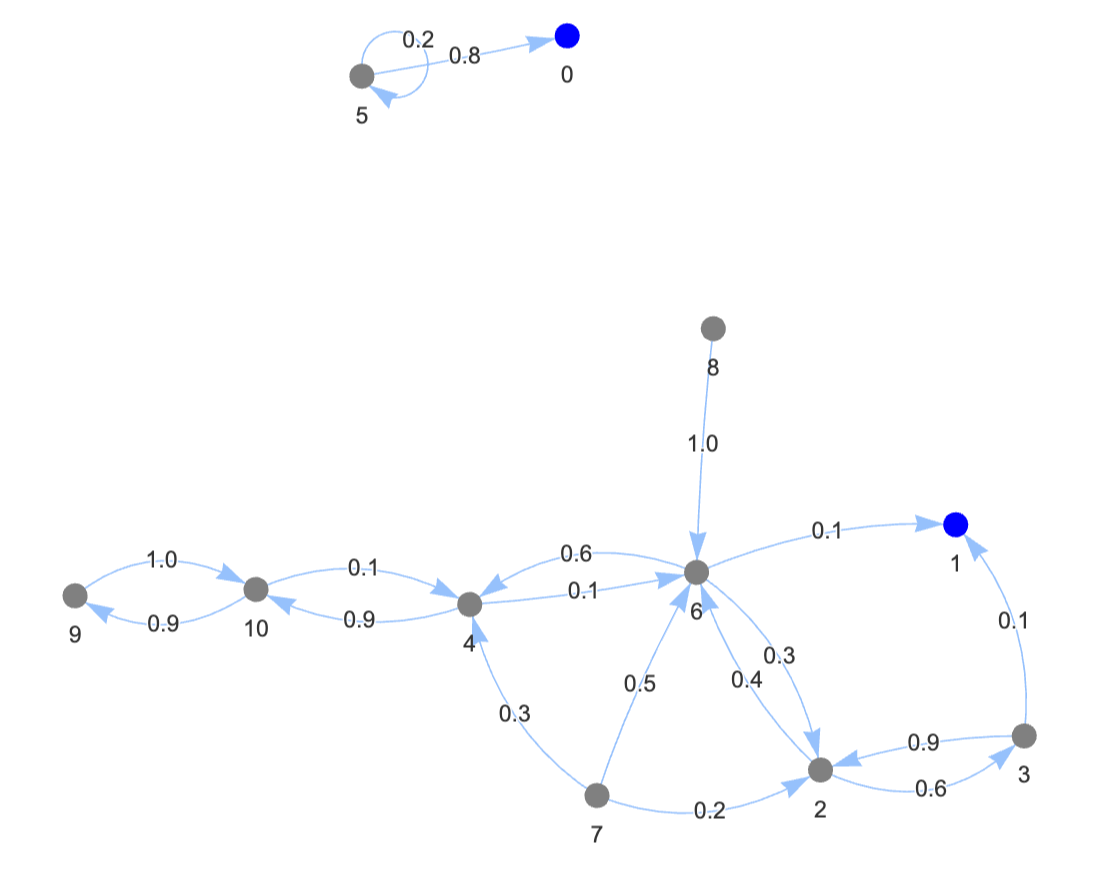
\includegraphics[width=\textwidth]{11_random}}
        \caption{11 nodes}
        \label{subfig:random-11and12-11}
    \end{subfigure}
    \hfill
    \begin{subfigure}[t]{0.45\textwidth}
        \centering
        \fbox{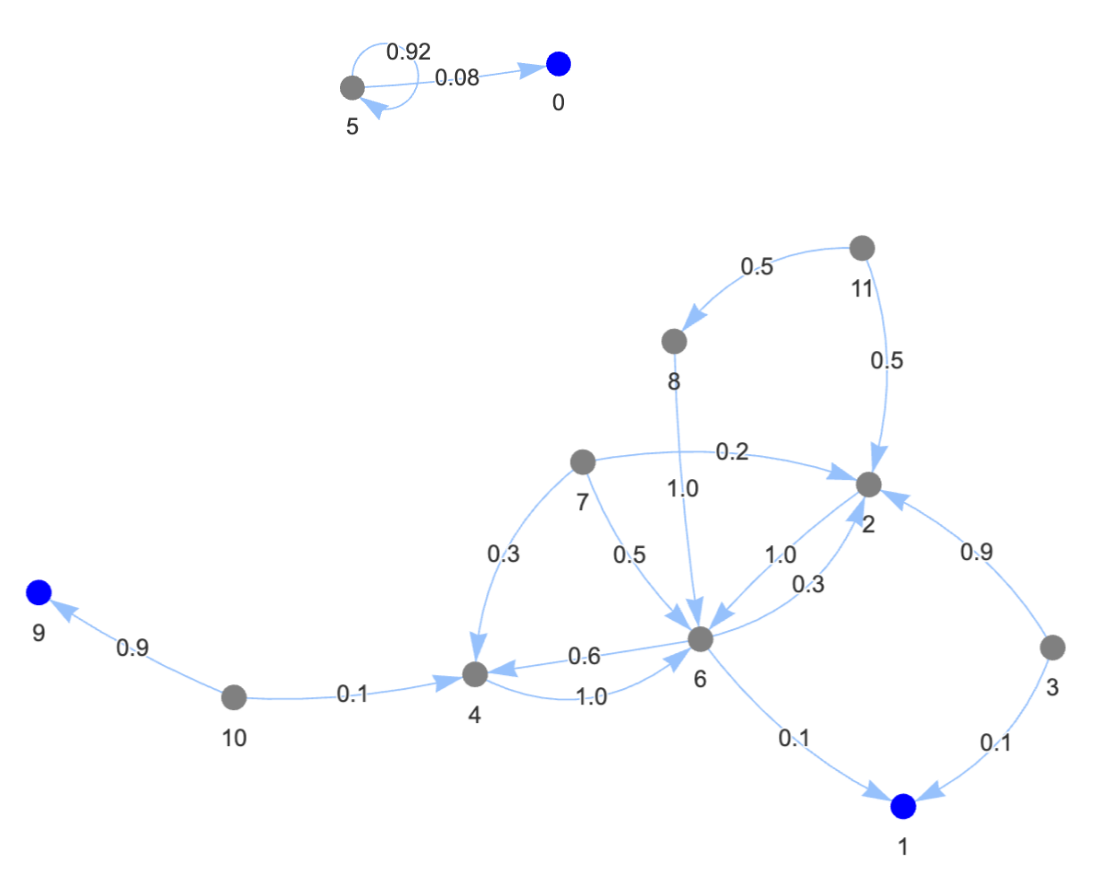
\includegraphics[width=\textwidth]{12_random}}
        \caption{12 nodes}
    \end{subfigure}
    \caption{Delegation graphs with 11 and 12 nodes (Blue nodes are sinks)}
    \label{fig:random-11and12}
\end{figure}

Inspecting the graphs reveals a possible explanation for this behavior. When the graph has 12 nodes, node \texttt{9} is a sink, while in the graph with 11 node it delegates its power back to node \texttt{10}. In the latter case, power going out of node \texttt{9} needs to pass to node \texttt{10}, \texttt{4} and \texttt{6} before reaching a sink. While passing through node \texttt{4}, we can see that 90\% of the power is delegated back into the cycle between nodes \texttt{4}, \texttt{10} and \texttt{9}. The algorithm will iterate power through this loop, until enough has been drained out for the \texttt{total\_change} to fall below the cutoff. 

This is an important shortcoming of the iterative algorithm. Power can easily get trapped within permissible delegation cycles that only have a small drain allowing the power to escape from the cycle. Each iteration, if a great proportion of the nodes with draining edges' power is sent back into a cycle, the algorithm needs to continuously iterate until the power is back at the drain nodes, however depending on the cycle this may happen very inefficiently. This phenomenon will be tested more in \cref{subsec:cycles_draining}

\subsection{Large Graphs}

Delegation graphs may grow arbitrarily large. National elections for example can contains up to hundreds of millions of participants. This section explores how the algorithms perform when having to resolve graphs with a lot of nodes. Again, the graphs will be randomly generated, such that each nodes has between 0 and 3 delegates. 

\begin{figure}[t]
    \centering
    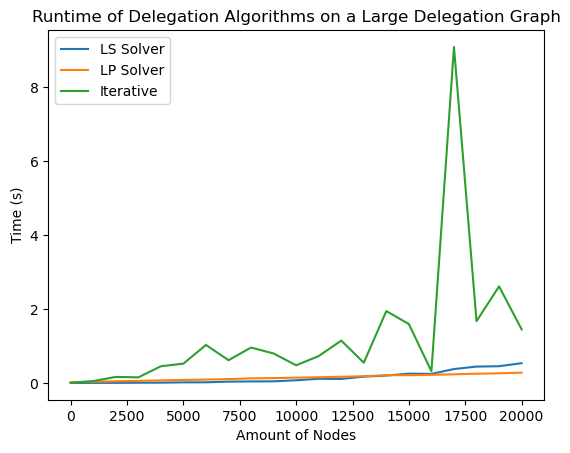
\includegraphics[width=0.4\textwidth]{0-20000_random}
    \caption{Runtime of delegation algorithms on a randomly generated delegation graph.}
    \label{fig:random-large}
\end{figure}

In \cref{fig:random-large} we can see, that it is difficult to determine a pattern in the runtime for the iterative algorithm. Depending on the underlying delegation graph, the runtime can grow unpredictably large. What is evident from the runtime graph however, is that in as the graphs get larger its runtime never subceeds the runtimes of the other two algorithms, while it is worth mentioning that for some graphs, the iterative algorithm's runtime is not a lot longer than that of the other two algorithms. It is difficult to make any statement about the runtime class of the iterative algorithm based just on the number of nodes in the graph, since, depending on the structure of the graph and the cutoff value the runtime can get arbitrarily high. The comparatively high runtime of the iterative algorithm overshadows the runtimes of the other two, so in order to better discuss and analyze their performance, \cref{fig:random-large-no-iterative} shows the same graph as in \cref{fig:random-large}, without the runtimes for the iterative algorithm.

\begin{figure}[t]
    \centering
    \begin{subfigure}[t]{0.45\textwidth}
        \centering
        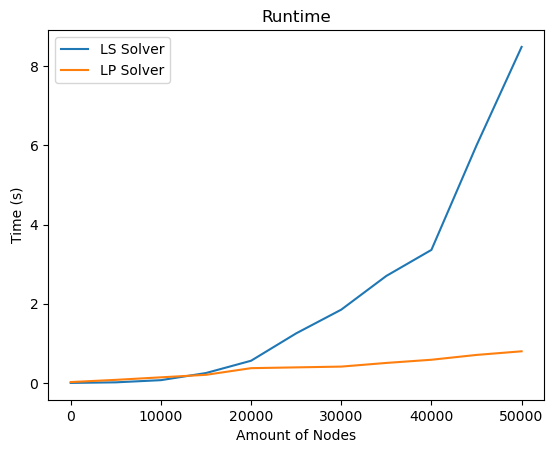
\includegraphics[width=\textwidth]{0-50000_random_no_iterative}
        \caption{Linear scale}
         \label{subfig:random-large-no-iterative-linear}
    \end{subfigure}
    \hfill
    \begin{subfigure}[t]{0.45\textwidth}
        \centering
        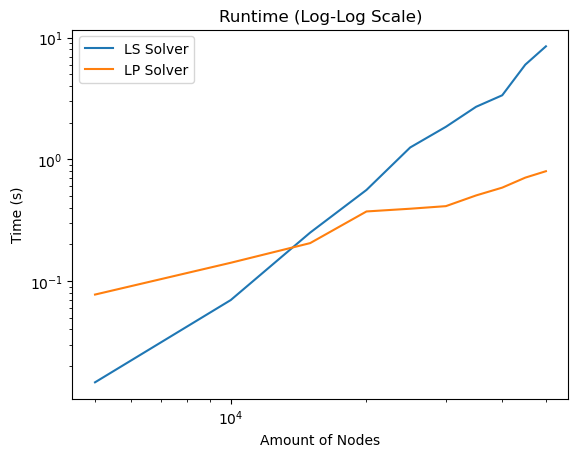
\includegraphics[width=\textwidth]{0-50000_random_no_iterative_loglog}
        \caption{Loglog scale}
         \label{subfig:random-large-no-iterative-loglog}
    \end{subfigure}
    \caption{Runtime of delegation algorithms on a randomly generated delegation graph.}
    \label{fig:random-large-no-iterative}
\end{figure}

\begin{figure}[t]
    \centering
    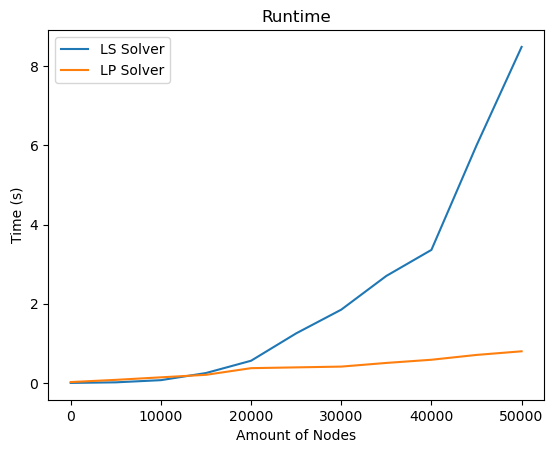
\includegraphics[width=0.4\textwidth]{0-50000_random_no_iterative}
    \caption{Runtime of delegation algorithms on a randomly generated delegation graph.}
    \label{fig:random-large-no-iterative}
\end{figure}

\Cref{subfig:random-large-no-iterative-linear} shows, that as the delegation graph grows, the LP solver's runtime grows more slowly than the LS Solver's. For resolving smaller graphs, the LS solver outperforms the LP solver, with a runtime of almost zero for empty or very small graphs, while the LP solver has a clearly non-zero runtime even for very small graphs. However, at around 12 000 nodes, this changes, as the LP solver's runtime's slower growth catches up with that of the LS solver. 

The type of growth, so the runtime class, is not immediately clear from the graphs, although the LP solver's growth seems to be more linear than that of the LS solver. Looking at the same results on a loglog graph reveals, that the LS solvers runtime may follow a power law.

Fitting the data into different kinds of curves reveals, that the LP implementations runtime likely has linear growth, while the LS solver grows following a power distribution, such that it is in the runtime class of $O(n^{2.778})$.

\TODO{Put the runtime results and/or the code and the regression results into the annex, or into the text...}

\subsection{Dense Graphs}

While we expect most delegators in any delegation graph to only delegate to a handful of people, a well formed delegation graph can have any number of delegates per delegator. Thus, it is also interesting to compare how the three algorithms compare when resolving more dense graphs. In this section, we test the three implementations on NetworkX's $G_{n,p}$ graph generator \texttt{gnp\_random\_graph}, which returns a directed graph with $n$ nodes, where each node connected to each other node with probability $p$, which is set to $0.5$ for the remainder of this section \cite{hagbergExploringNetworkStructure2008}. These graphs are not well-formed delegation graphs out-of-the box, thus we adapt them by removing outgoing edges of nodes, turning them into sinks, until 10\% of the nodes are sinks. Then, each delegators vote is equally distributed to all of its outgoing edges, such that the edge weights add up to 1. Finally, any closed delegation cycles are removed by removing a random edge in the cycle (and re-normalizing the edge weights). 

\begin{figure}[t]
    \centering
    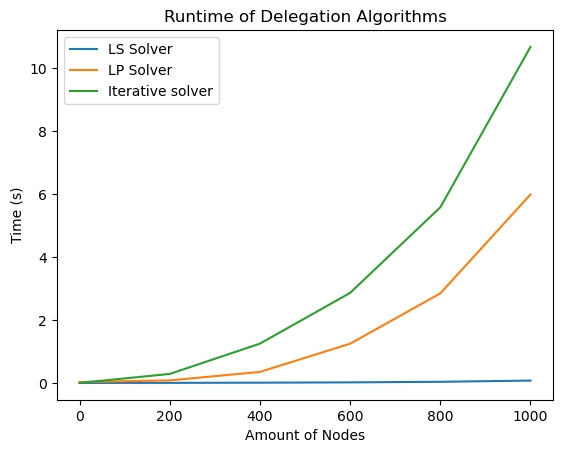
\includegraphics[width=0.4\textwidth]{0-1000_dense}
    \caption{Runtime of delegation algorithms on a randomly generated delegation graph.}
    \label{fig:dense-small}
\end{figure}

\Cref{fig:dense-small} shows the runtime of these three algorithms. The runtime of the iterative algorithm lacks the spikes found when resolving sparse graphs. This is likely due to the nature of the graphs we create. Every delegator is connected to half of all other nodes ($p = 0.5$), and of these $10\%$ are sinks, thus power drains quickly into sinks, and situations where power iterates a long time without seeing a sink are less frequent. Regardless, the iterative algorithm exhibits the worst runtime of the three. 

\begin{figure}[t]
    \centering
    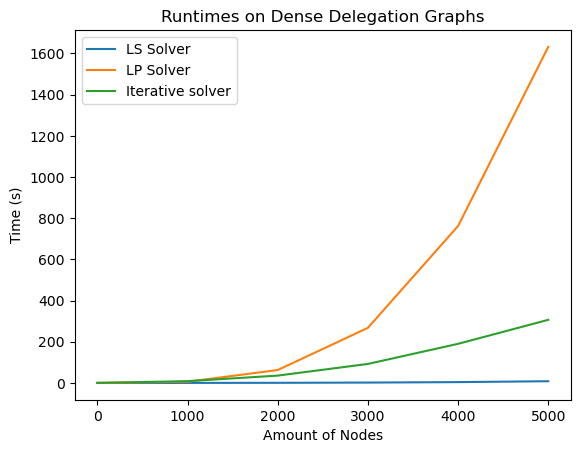
\includegraphics[width=0.4\textwidth]{0-5000_dense}
    \caption{Runtime of delegation algorithms on a randomly generated delegation graph.}
    \label{fig:dense-large}
\end{figure}

Testing the three algorithms on larger dense graphs, reveals surprisingly, that the LP solver's runtime is considerably worse than that of both the iterative and LS solver. A dense graph with 5,000 nodes, and thus about 125,000 delegations, takes the LS solver only about 12 seconds, the iterative solver 445 seconds, and the LP solver almost 2,400 seconds. Even though the LS solver is optimized for sparse matrices, it outperforms the other two implementations on dense graphs.

\subsection{Cycles Which Retain a Lot of their Power}

\label{subsec:cycles_draining}

\begin{figure}[t]
	\centering
	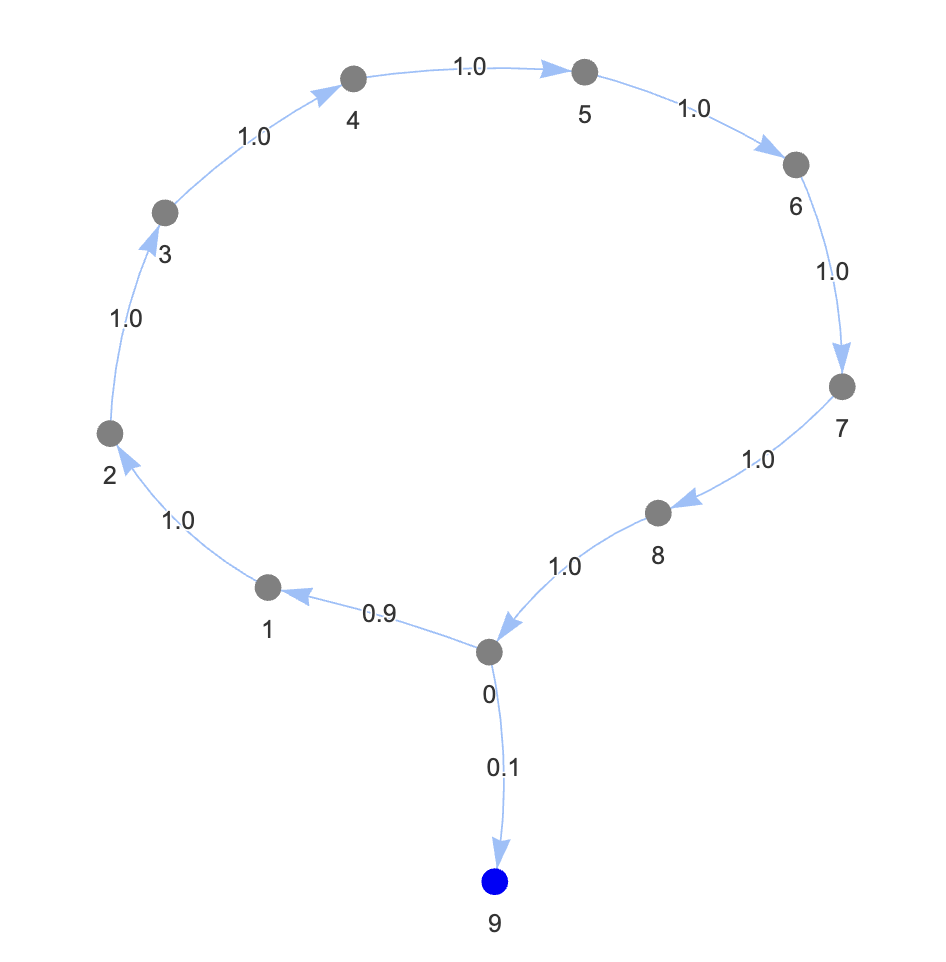
\includegraphics[width=0.4\textwidth]{big_cycle_example}
	\caption{An example of the cycles used for the benchmarks. The blue node is the sink}
	\label{fig:big_cycle_example}
\end{figure}

To further explore one of the iterative algorithm's shortcomings, this section will explore and compare runtime behavior for delegation cycles which are not closed, but contain only few, weak edges for power to drain, thus forcing power to iterate around in the cycle before it reaches a sink. Specifically, we construct graphs with delegates all delegating power to the next node in the cycle. One node in the cycle contains an edge with weight 0.1 to a sink, while the other 0.9 of its power go to the first node in the cycle. \Cref{fig:big_cycle_example} contains an exemplary image of such a graph with 10 nodes. 

\begin{figure}[t]
    \centering
    \begin{subfigure}[t]{0.45\textwidth}
    	\centering
    	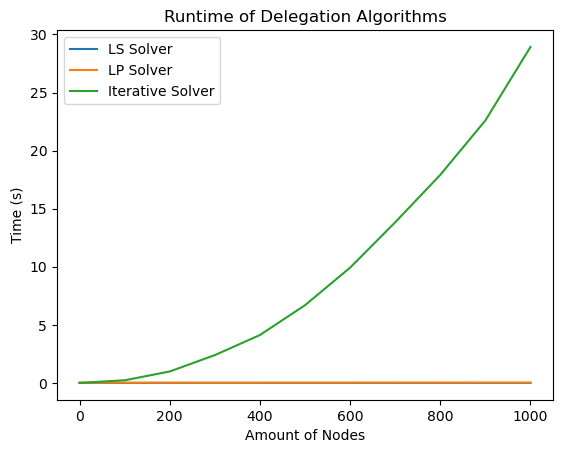
\includegraphics[width=\textwidth]{0-1000_cycle}
    	\caption{Linear scale}
    	\label{subfig:cycle-small-linear}
    \end{subfigure}
    \hfill
    \begin{subfigure}[t]{0.45\textwidth}
        \centering
        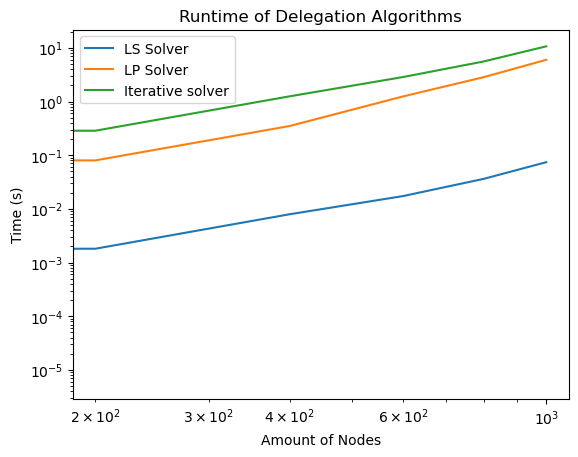
\includegraphics[width=\textwidth]{0-1000_dense_loglog}
        \caption{Loglog scale}
         \label{subfig:cycle-small-loglog}
    \end{subfigure}
    \caption{Runtime of delegation algorithms on a randomly generated delegation graph.}
    \label{fig:cycle_small}
\end{figure}

The runtimes in \cref{subfig:cycle-small-linear} show, that as expected, the iterative algorithm struggles considerably with the resolution of these graphs, while the other two algorithms exhibit behavior similar to that on randomly generated sparse delegation graphs. The growth of the runtimes seems to be polynomial, with the iterative algorithm belonging to the runtime class $O(n^{2.12})$. Being able to resolve these kinds of loops is one of the greatest strength of the two approaches, which don't simulate power as flow through the graph. By directly solving the system of linear equations, they are a lot more well equipped to deal with this specific corner case.  

\begin{figure}[t]
	\centering
    	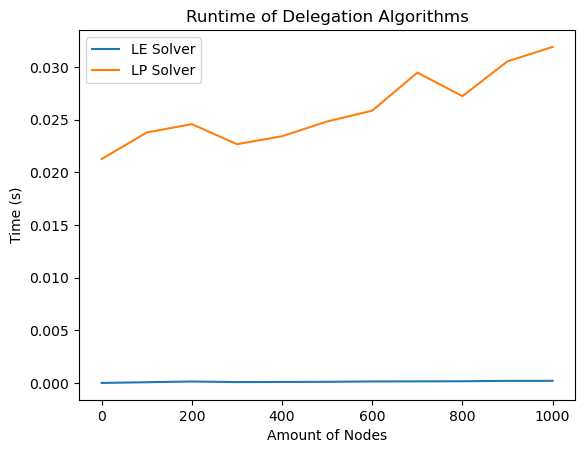
\includegraphics[width=0.4\textwidth]{0-1000_cycle_no_iterative}
    	\caption{Runtime of delegation algorithms on a randomly generated delegation graph.}
	\label{fig:cycle-small-no-iterative-linear}
\end{figure}

As seen in \cref{fig:cycle-small-no-iterative-linear}, which shows the same graph as in \cref{subfig:cycle-small-linear} without the iterative algorithm's runtime, the runtime of the LS and LP Solvers grows similarly to when resolving randomly generated (sparse) delegation graphs, such as the ones found in \cref{subsec:small_graphs}.

Such a cycle as the one we deliberately constructed is not the only situation in which the iterative algorithm will struggle. As long as power is not efficiently funneled toward a sink, the iterative algorithm will have to spend more time moving the power around until enough has drained into a sink for \texttt{total\_change} to fall below the cutoff value. A further example of such behavior is the cycle that caused runtime to spike in \cref{subfig:random-11and12-11}. An artificial example of this situation is shown below in \cref{fig:big_cycle_example}.

\section{Social Graphs}

Social graphs provide an excellent way to \TODO{Finish this sentence}... We will use them to create sample delegation graphs based on social behaviors, which can predict ways humans may delegate if given the chance to delegate fractionally. These graphs are still only based on models, however since they are artificial, we can scale them and explore how the algorithms scale.

\subsection{Small World Graphs}

\TODO{Introduce those woganotiz stroff Small World graphs and the way I generated them (with prepare\_graph 20\% sinks, etc.)}

\begin{figure}[t]
    \centering
    \begin{subfigure}[t]{0.45\textwidth}
        \centering
        \fbox{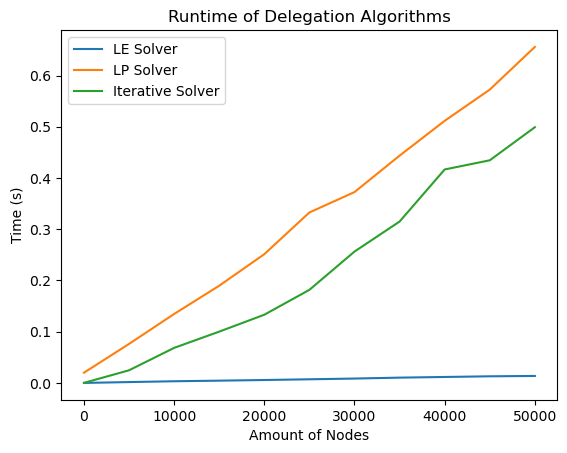
\includegraphics[width=\textwidth]{0-50000_small_world}}
        \caption{Linear scale}
        \label{subfig:small_world_graph_linl}
    \end{subfigure}
    \hfill
    \begin{subfigure}[t]{0.45\textwidth}
        \centering
        \fbox{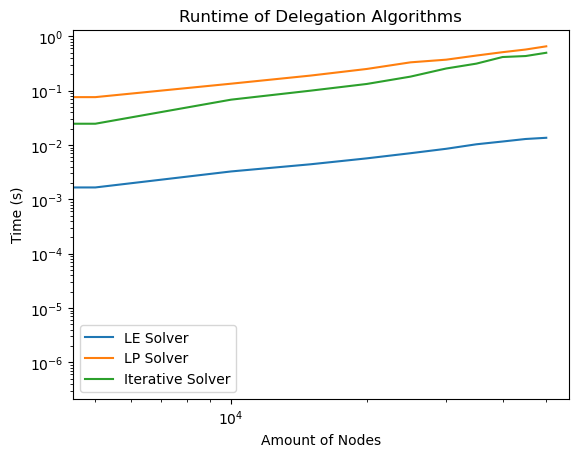
\includegraphics[width=\textwidth]{0-50000_small_world_loglog}}
        \caption{Loglog scale}
        \label{subfig:small_world_graph_loglog}
    \end{subfigure}
    \caption{Runtime of delegation algorithms on a randomly generated delegation graph.}
    \label{fig:small_world_graph}
\end{figure}

Fig XX shows the results of the benchmarks on these graphs. 

\subsection{R-Mat Graphs}

Another method for generating artificial social graphs is the R-MAT (Recursive Matrix) model. \TODO{cite \url{https://epubs.siam.org/doi/pdf/10.1137/1.9781611972740.43}} This model requires four parameters—$a$, $b$, $c$, and $d$—which are probabilities that sum to one, as well as the desired number of nodes $N$ and edges $M$. The algorithm begins with an empty $\sqrt{N} \times \sqrt{N}$ adjacency matrix, where a nonzero entry at position $(i, j)$ indicates a directed edge from node $i$ to node $j$. To determine where to place each edge, the matrix is recursively subdivided into four quadrants, with the probability of selecting a quadrant governed by the parameters $a$, $b$, $c$, and $d$. This recursive partitioning continues until a single cell ($1 \times 1$) is reached, and an edge is added at that location. The process is repeated until all $M$ edges have been assigned.




\section{Real-World Datasets}

This section evaluates the three algorithms on some real-world datasets. While liquid democracy without fractional delegation has been implemented and tested in studies \TODO{Cite}, to the authors knowledge there are no datasets for authentic fractional delegations. As an alternative, we have fallen back to transforming datasets which may resemble fractional delegations into delegation graphs. We  introduce the three datasets individually, followed by a joint evaluation in \cref{subsec:datasets_eval}.

\subsection{Epinions}

Epinions.com is a "general consumer review site", in which members can decide whether to "trust" each other. \TODO{cite: \url{https://snap.stanford.edu/data/soc-Epinions1.html}} The Stanford Network Analysis Project (SNAP) provides a web-of-trust graph generated from this relations. \TODO{cite: \url{https://snap.stanford.edu/data/soc-Epinions1.html}} The graph is directed and unweighted, thus an existing edge implies trust, and a missing edge implies the lack thereof.

After turning the graph into a delegation graph (see pipeline in fig XX), with the $n\%$ sink threshold set to zero, so the algorithm does not add any new sinks to the graph by removing outgoing edges of nodes, we observe the following statistics for the delegation graph, which will be called the Epinions Graph. The Epinions Graph contains 75139 nodes, of which about 0.21\% are sinks. \Cref{subfig:epinions_outdegrees} shows the distribution of outdegrees in the Epinions Graph, outdegree meaning the amount of outdoing edges of a node. The mean outdegree is 6.76.

330 closed delegation cycles were collapsed, which affected 740 nodes, about 0.01\% of nodes in the graph. Interestingly, most powerful node after resolving is the "lost" node, so the node where power goes, that was delegated into closed delegation cycles. The total amount of power lost adds up to 2777.056087, which accounts for about 0.037\% of power in the graph. The distribution of powers after resolving is shown in \cref{subfig:epinions_powers}.

\TODO{Fix and make more clean the captions for runtime graphs. Currently they mention "delegation algorithms", which is outdated terminology}

\subsection{Bitcoin OTC Trust Network}

Users trading Bitcoin on the platform "Bitcoin OTC" maintain a record of trust to other users, in order to prevent transactions with untrustworthy users. SNAP provides the Bitcoin OTC Trust Graph, a graph of this trust between users. \TODO{cite: \url{https://snap.stanford.edu/data/soc-sign-bitcoin-otc.html}} The graph is directed and weighted, with weights ranging from -10 to 10, total distrust to total trust. \TODO{cite: \url{https://snap.stanford.edu/data/soc-sign-bitcoin-otc.html}} 

The graph was first cleaned, to remove all edges with a non-positive trust values, before being turned into a delegation graph as per fig XX, again not adding any sinks artificially. The preprocessing pipeline normalises edge weights, meaning outgoing trust levels are scaled down proportionally to add up to one, preserving relative differences in trust. The finished graph contains 5573 nodes, of which about 0.15\% are sinks. The outdegree distribution in the Bitcoin OTC Trust Graph is shown in \cref{subfig:bitcoinotc_outdegrees}.

During the preprocessing of this graph, 43 of the graph's 5573 nodes were to be removed since they were in a closed delegation cycle. About 111.2 units of power were lost to closed delegation cycles,  0.02\% of the total power in the graph. The distribution of powers after resolving is shown in \cref{subfig:bitcoinotc_powers}

\subsection{Slashdot Zoo}

The Slashdot technology news size has a so-called "zoo" feature, in which users can tag other users as friends and foes. \TODO{Cite: \url{https://dai-labor.de/en/publications/the-slashdot-zoo-mining-a-social-network-with-negative-edges/}} The Distributed AI Laboratory in Berlin (DAI Labor) provides a graph based on this data. \TODO{Cite: \url{https://dai-labor.de/en/publications/the-slashdot-zoo-mining-a-social-network-with-negative-edges/}} It is a directed and weighted graph, where an edge weight of +1 indicates a friend relationship, and an edge weight of -1 indicates a foe relationship.

This graph was also cleaned to only contain positive edges and turned into a delegation graph, again not adding any sinks artificially. The delegation graph contains 69995 edges, of which about 0.4\% are sinks. The outdegree distribution in this graph is shown in \cref{subfig:slashdot_outdegrees}.

1061 nodes were removed due to being in a closed delegation cycle...

\TODO{continue this once I am more sure what I should actually include.}
 
 \subsection{Evaluation of the datasets}
 \label{subsec:datasets_eval}

 \begin{figure}[t]
    \centering
        \begin{subfigure}[t]{0.30\textwidth}
        \fbox{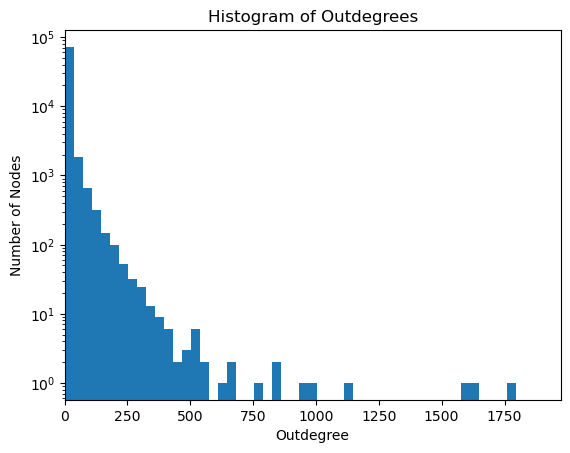
\includegraphics[width=\textwidth]{epinions_outdegree_distr}}
        \caption{Epinions Dataset}
        \label{subfig:epinions_outdegrees}
    \end{subfigure}
    \hfill
        \centering
        \begin{subfigure}[t]{0.30\textwidth}
        \fbox{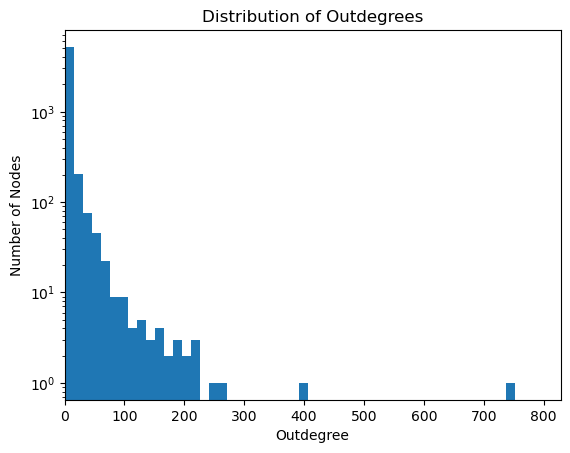
\includegraphics[width=\textwidth]{bitcoinotc_outdegree_distr}}
        \caption{Bitcoin OTC Dataset}
        \label{subfig:bitcoinotc_outdegrees}
    \end{subfigure}
    \hfill
    \begin{subfigure}[t]{0.30\textwidth}
    	\centering
    	\fbox{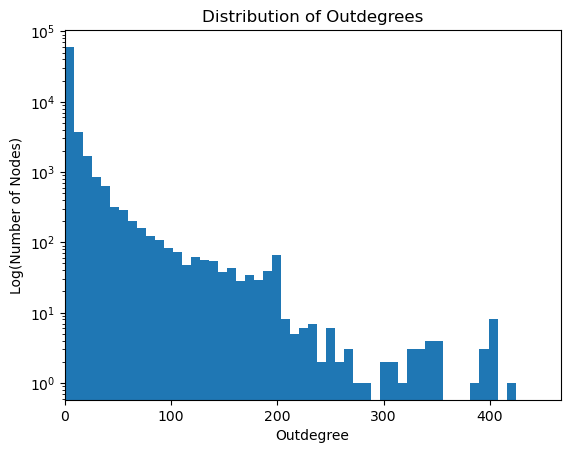
\includegraphics[width=\textwidth]{slashdot_outdegree_distr}}
    	\caption{Slashdot Zoo Graph.}
	\label{subfig:slashdot_outdegrees}
    \end{subfigure}
    \caption{Distribution of outdegrees}
    \label{fig:datasets_outdegree_distr}
\end{figure}

 \begin{figure}[t]
    \centering
        \begin{subfigure}[t]{0.30\textwidth}
        \fbox{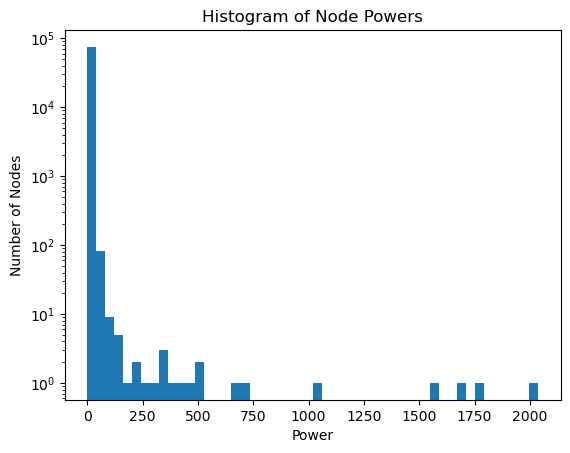
\includegraphics[width=\textwidth]{epinions_power_distr}}
        \caption{Epinions Dataset}
        \label{subfig:epinions_powers}
    \end{subfigure}
    \hfill
        \centering
        \begin{subfigure}[t]{0.30\textwidth}
        \fbox{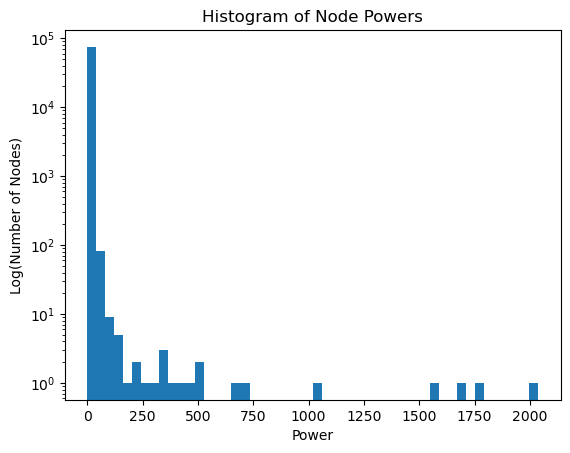
\includegraphics[width=\textwidth]{bitcoinotc_power_distr}}
        \caption{Bitcoin OTC Dataset}
        \label{subfig:bitcoinotc_powers}
    \end{subfigure}
    \hfill
    \begin{subfigure}[t]{0.30\textwidth}
    	\centering
    	\fbox{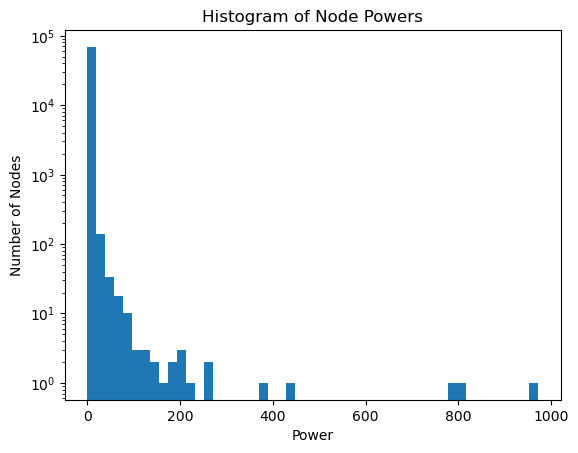
\includegraphics[width=\textwidth]{slashdot_power_distr}}
    	\caption{Slashdot Zoo Graph.}
	\label{subfig:slashdot_powers}
    \end{subfigure}
    \caption{Distribution of powers}
    \label{fig:datasets_powers}
\end{figure}

 \begin{figure}[t]
    \centering
        \begin{subfigure}[t]{0.30\textwidth}
        \fbox{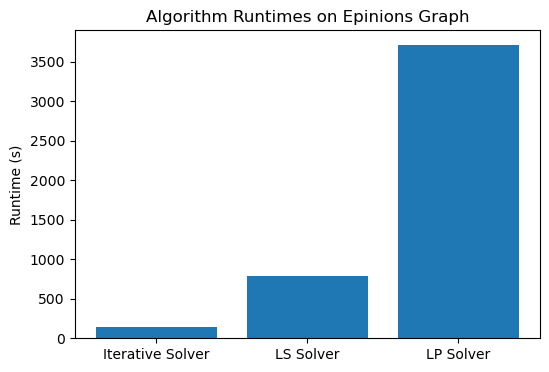
\includegraphics[width=\textwidth]{epinions_dataset}}
        \caption{Epinions Dataset}
    \end{subfigure}
    \hfill
        \centering
        \begin{subfigure}[t]{0.30\textwidth}
        \fbox{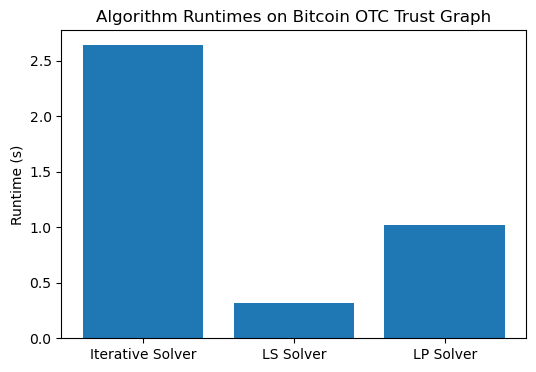
\includegraphics[width=\textwidth]{bitcoinotc_dataset}}
        \caption{Bitcoin OTC Dataset}
    \end{subfigure}
    \hfill
    \begin{subfigure}[t]{0.30\textwidth}
    	\centering
    	\fbox{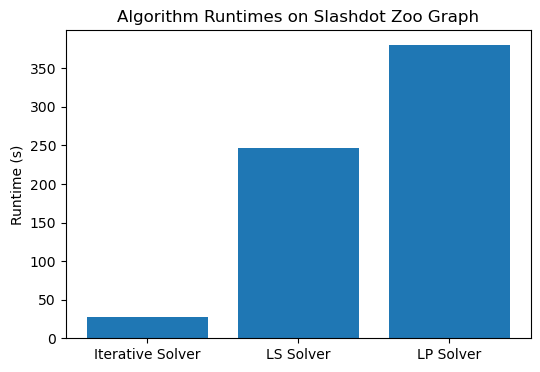
\includegraphics[width=\textwidth]{slashdot_dataset}}
    	\caption{Slashdot Zoo Graph.}
    \end{subfigure}
    \caption{Runtimes}
    \label{fig:datasets_runtimes}
\end{figure}


\TODO{Maybe mention also at some point, that this evaluation is a comparison between different solvers for systems of linear equations}

\TODO{Mention that the iterative solver is a lot less precise}